\chapter{Design Architecture}
\label{chp:design}
% Talk about previous designs and why I didn't/couldn't choose them (continuous tracking and sending to server).
As discussed in \nameref{it:1} in \autoref{it:1}, the non-continuous server design was chosen. The continuous server would be more complex to design and implement than the non-continuous version. This is because a constant connection between the plugin and server was required. If the network connection was interrupted or disconnected then data would not be sent to the server. This means that a fail-safe protocol would have to be implemented, such as writing the unsent data to file. This fail-safe protocol implementation would be required for the non-continuous server anyway.

The server-side of the continuous design would also need to be more sophisticated. The server would have to know when a new project is being started, which project data is being received, and when a project is completed. The non-continuous server only required a method to submit the tracked data file.

The following pages show diagrams to aid with discussing the final design of the system.

\newpage

\section{Architecture Diagram}
\autoref{fig:architecture-diagram} shows the interaction between each of the modules. The plugin only needs to track file changes in the editor. This data is saved to an XML file, which the user can submit to the server using the front-end web application. This requires authentication using Aberystwyth credentials. Once the file has been submitted, the back-end server converts the XML data to JSON and stores it in the MongoDB database. The post-processor is continually monitoring the database for new student submissions to process and update the database with the result.

\vspace*{\fill}

\begin{figure}[H]
  \centering
  \fbox{
    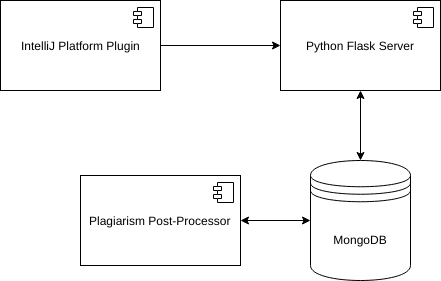
\includegraphics[height=\textheight,
    keepaspectratio=true,
    width=\textwidth,
    ]{figures/architecture-diagram.png}
  }
  \caption[Final design architecture diagram]{Architecture diagram}
  \label{fig:architecture-diagram}
\end{figure}

\vspace*{\fill}

\newpage

\section{Student Plugin Interaction Sequence Diagram}
\autoref{fig:sequence-diagram-student-plugin} shows a typical students' interaction with the plugin. Initially, when a student opens a project, the tracked files are checked for external changes. This is done by comparing each files last known contents (which is stored as a base 64 encoded value) with its current file contents. The difference is added to the list of changes for each file. A \texttt{DocumentListener} is then added to the project for listening to file changes. Each file change is identified and then added to the list of changes for that file. After every new change that is added, the files last known contents is updated (for checking external changes). The recorded data is saved any time a file is saved. File change tracking stops when the project is closed (or if the plugin is disabled or uninstalled).

\vspace*{\fill}

\begin{figure}[H]
  \centering
  \fbox{
    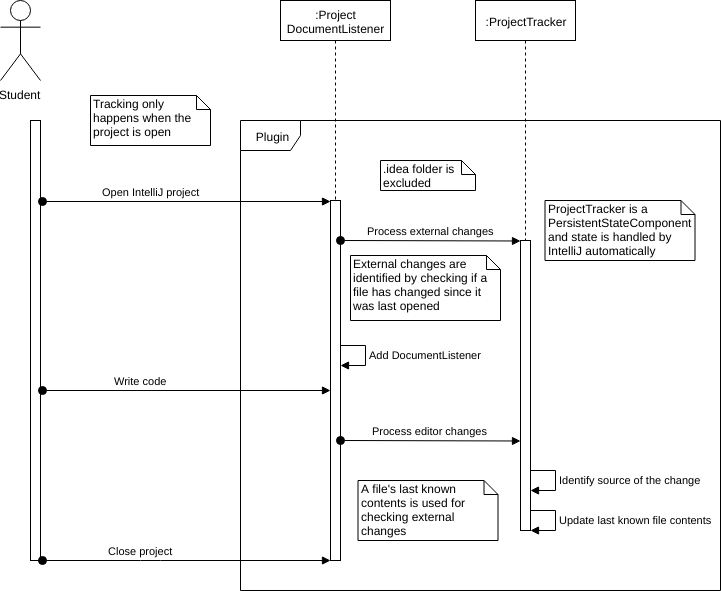
\includegraphics[height=\textheight,
    keepaspectratio=true,
    width=\textwidth,
    ]{figures/sequence-diagram-student-plugin.png}
  }
  \caption[Student-plugin sequence diagram]{Sequence diagram showing a student interacting with the IntelliJ plugin}
  \label{fig:sequence-diagram-student-plugin}
\end{figure}

\vspace*{\fill}

\newpage

\section{Student Server Interaction Sequence Diagram}
\autoref{fig:sequence-diagram-student-server} shows a students' interaction with the server. Once the project is completed. The student may login to the web application using their Aberystwyth University credentials. This authorisation is achieved using the LDAP server provided by Aberystwyth University. This requires the back-end server to be running on the Aberystwyth University network. The LDAP server returns if authentication was successful or not. If successful, then the student will be redirected to their dashboard. A query is sent to the database to retrieve all of the students' submissions. These submissions are then displayed in a table in the dashboard. Students can post new project submissions by uploading the XML file with additional meta data for identification in a form. The form is submitted via POST. The XML file is decrypted and added to the students submissions in the database. The user will be notified of success or failure via a flash message.

\vspace*{\fill}

\begin{figure}[H]
  \centering
  \fbox{
    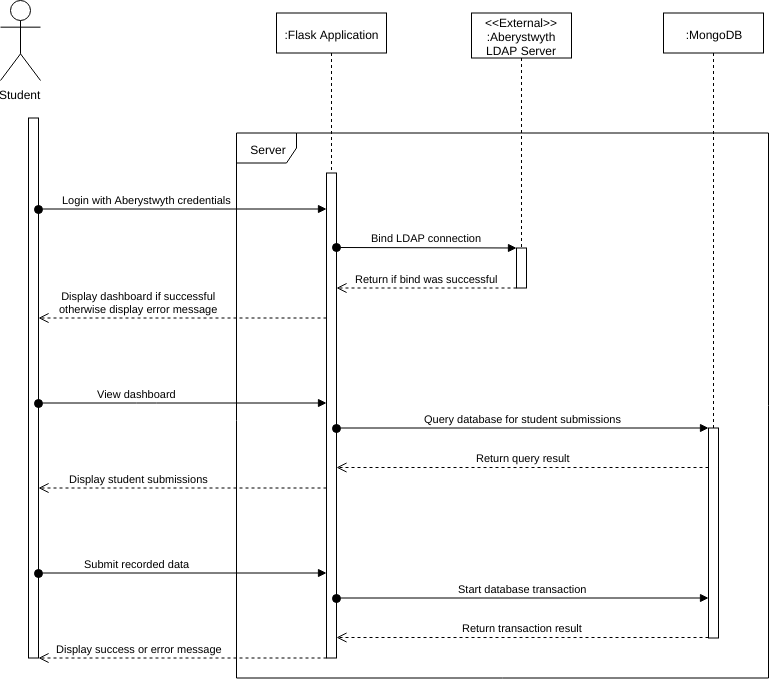
\includegraphics[height=\textheight,
    keepaspectratio=true,
    width=\textwidth,
    ]{figures/sequence-diagram-student-server.png}
  }
  \caption[Student-server sequence diagram]{Sequence diagram showing a student interacting with the server}
  \label{fig:sequence-diagram-student-server}
\end{figure}

\vspace*{\fill}

\newpage

\section{Post-Processor Sequence Diagram}
\autoref{fig:sequence-diagram-post-processor} shows when a student posts a new submission via the web application, the post-processor is notified. This is implemented using the \texttt{watch} method from PyMongo. The \texttt{watch} method notifies the post-processor of all changes in the database in real time. These changes must first be filtered to only identify new submissions. All new submissions are processed and then the resulting data is inserted back into the database using the original submission id and user id. See \autoref{chp:results} for an in-depth review about the post-processor results.

\vspace*{\fill}

\begin{figure}[H]
  \centering
  \fbox{
    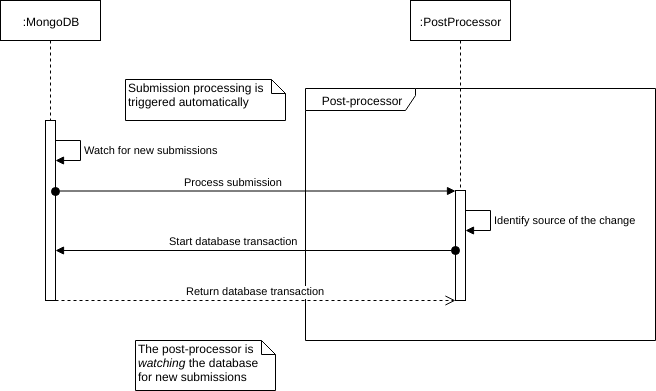
\includegraphics[height=\textheight,
    keepaspectratio=true,
    width=\textwidth,
    ]{figures/sequence-diagram-post-processor.png}
  }
  \caption[Post-processor sequence diagram]{Sequence diagram for the post-processor}
  \label{fig:sequence-diagram-post-processor}
\end{figure}

\vspace*{\fill}

\newpage

\section{Data Structure Class Diagram}
The main class that provides all the tracking is the \texttt{ProjectDocumentListener}. This class detects file changes, refactoring, and external file changes. When changes are detected they are added to the \texttt{ProjectTracker}. The \texttt{ProjectTracker} is used to store all of the changes for a single project. All file changes are stored in a Map data structure. The Map keys are the relative file paths as a String. The Map values are FileTracker objects. The \texttt{ProjectTracker} is also responsible for saving the state of the tracked changes by implementing \texttt{PersistentStateComponent}. An inner class, \texttt{CipherState} is used to store the encrypted Map data. The Map keys are not encrypted but the values are encrypted with 128-bit AES and base64 encoded. \texttt{CipherState} is used to load and save the state. Each tracked file has an associated \texttt{FileTracker} object. This object is used to store each files' Change list and cache. The file cache is its last known contents which is used for detecting external changes. The list of Changes can be used to reconstruct the file and compared with its cache.

\vspace*{\fill}

\begin{figure}[H]
  \centering
  \fbox{
    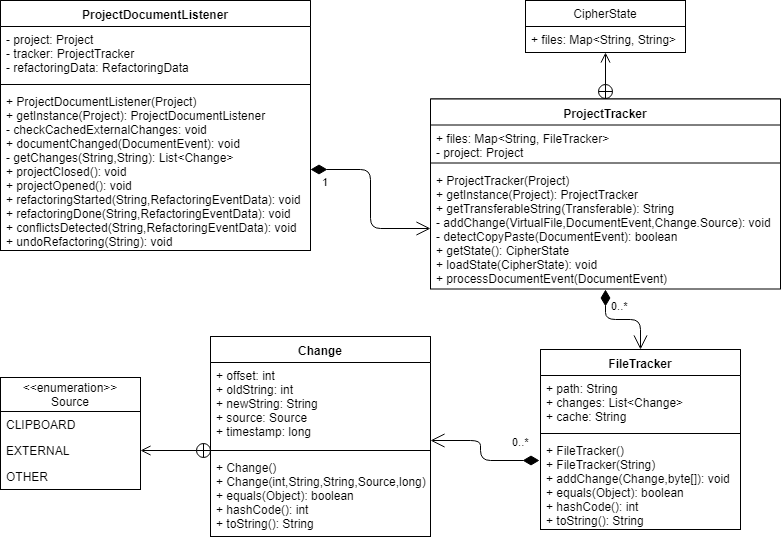
\includegraphics[height=\textheight,
    keepaspectratio=true,
    width=\textwidth,
    ]{figures/plugin-uml-class-diagram.png}
  }
  \caption[Tracked data structure]{Data structure to store tracked data}
  \label{fig:tracked-data-uml-class}
\end{figure}

\vspace*{\fill}

\newpage

\section{Front-end Web Application}
The approach used for designing the front-end web application was based off of bootstrap templates. The sign-in page is very simple, containing a simple form to enter credentials.

\begin{figure}[H]
  \centering
  \fbox{
    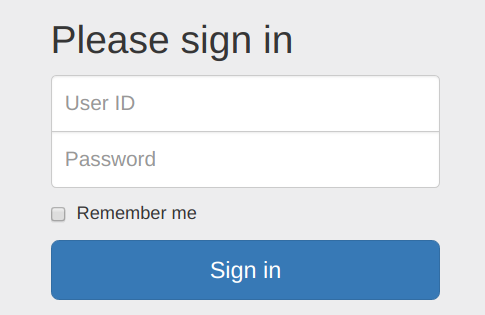
\includegraphics[height=.6\textheight,
    keepaspectratio=true,
    width=.6\textwidth,
    ]{figures/05-web-sign-in.png}
  }
  \caption[Web Sign-in Page]{The index page of the web-application. This is where users sign-in.}
  \label{fig:web-sign-in-page}
\end{figure}

After successful authentication, the user is redirected to the appropriate dashboard. Staff and students have separate dashboards. This is to display different data to each. Students will only see their previous submissions and be able to post new submissions as shown in \autoref{fig:web-student-dashboard}. Staff will be able to view all students submissions and more in-depth details as shown in \autoref{fig:web-staff-dashboard}. The staff submissions table contains three extra columns. The student name, details hyperlink, and P value. The student name is to identify the owner of the submission. The details link is to view further details of the submission. The P value is the calculated plagiarism value with its associated colour to ease with identification of possible plagiarism cases.

\begin{figure}[H]
  \centering
  \fbox{
    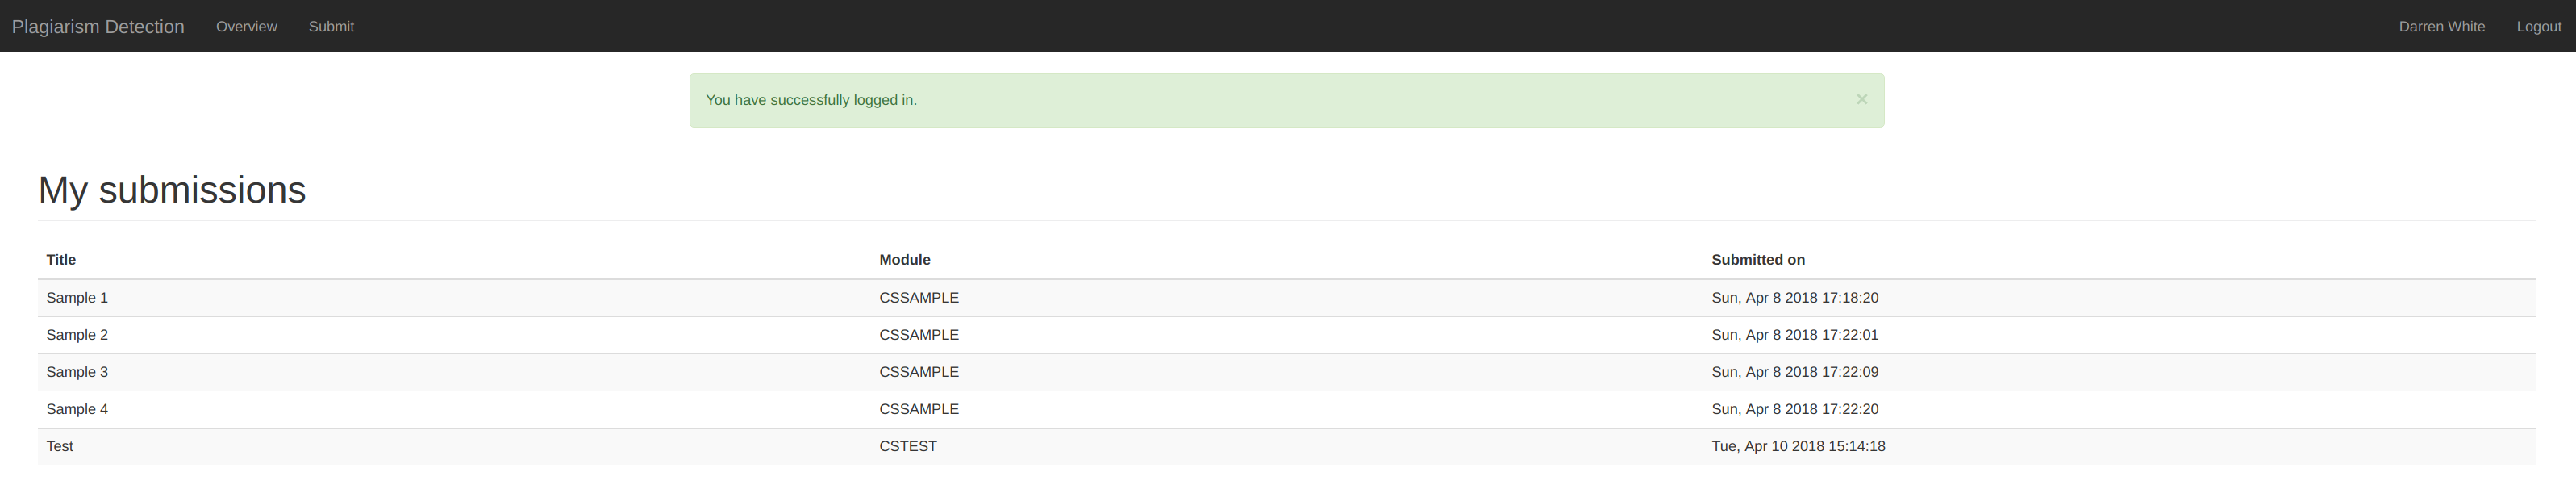
\includegraphics[height=\textheight,
    keepaspectratio=true,
    width=\textwidth,
    ]{figures/07-web-sign-in-success.png}
  }
  \caption[Web Student Dashboard Page]{The dashboard page of the web-application for students.}
  \label{fig:web-student-dashboard}
\end{figure}

\begin{figure}[H]
  \centering
  \fbox{
    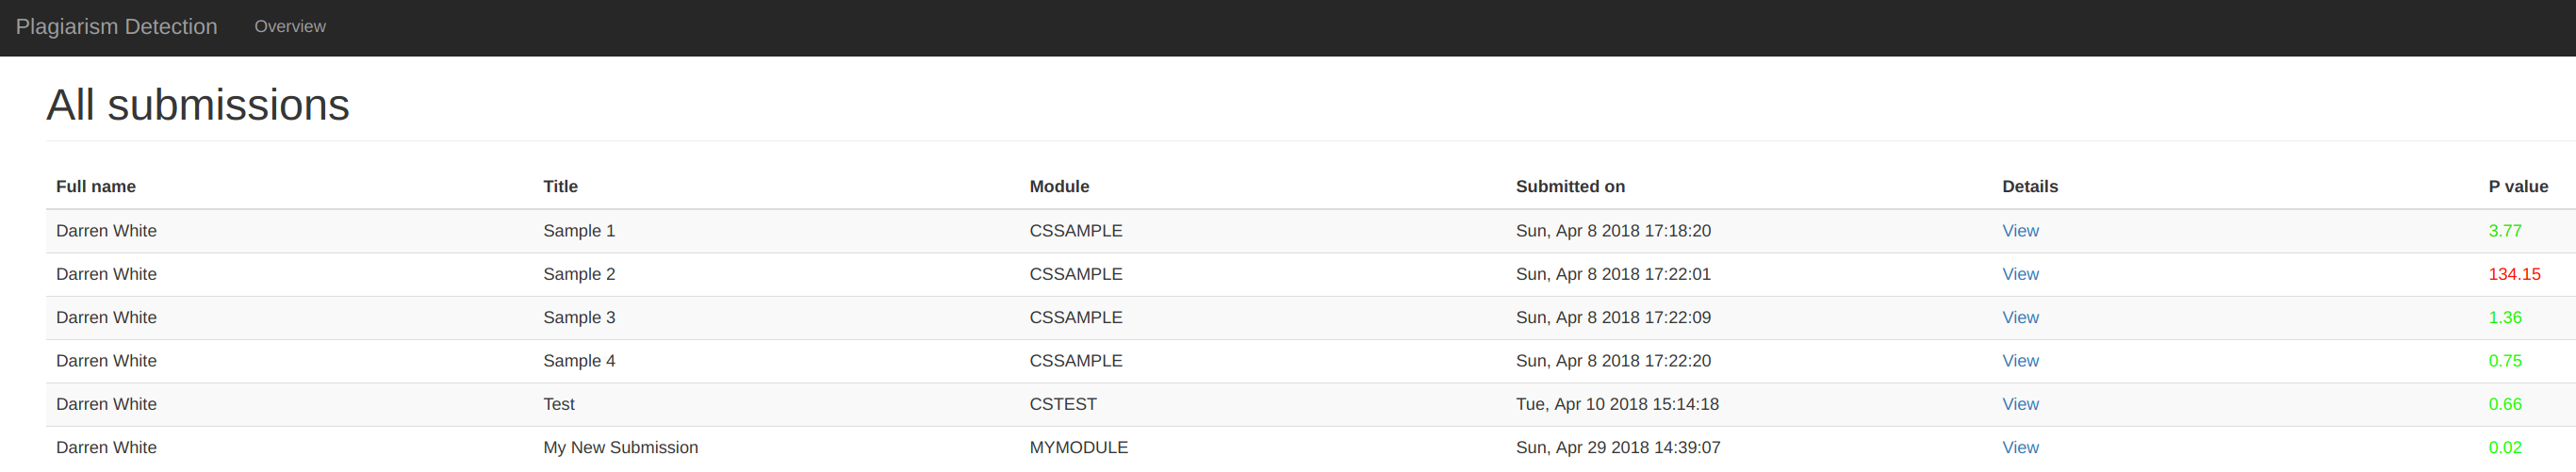
\includegraphics[height=\textheight,
    keepaspectratio=true,
    width=\textwidth,
    ]{figures/10-web-all-submissions.png}
  }
  \caption[Web Staff Dashboard Page]{The dashboard page of the web-application for staff.}
  \label{fig:web-staff-dashboard}
\end{figure}

Staff users are able to view submission details. This includes individual metrics from the post-processor, student submission details, FTS chart, and large changes. \autoref{fig:web-submission-details-data}, \autoref{fig:web-submission-details-chart}, and \autoref{fig:web-submission-details-changes} show the submission details information displayed on the page. All of this data can be used to help with identifying plagiarism. This is discussed more in-depth in \autoref{chp:results}.

\begin{figure}[H]
  \centering
  \fbox{
    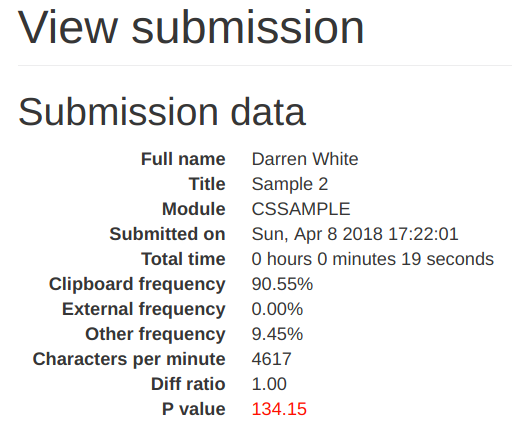
\includegraphics[height=.5\textheight,
    keepaspectratio=true,
    width=.5\textwidth,
    ]{figures/11-web-view-bad-submission-data.png}
  }
  \caption[Web Submission Data]{An example submission metrics view. This shows the submissions post-processed results.}
  \label{fig:web-submission-details-data}
\end{figure}

\begin{figure}[H]
  \centering
  \fbox{
    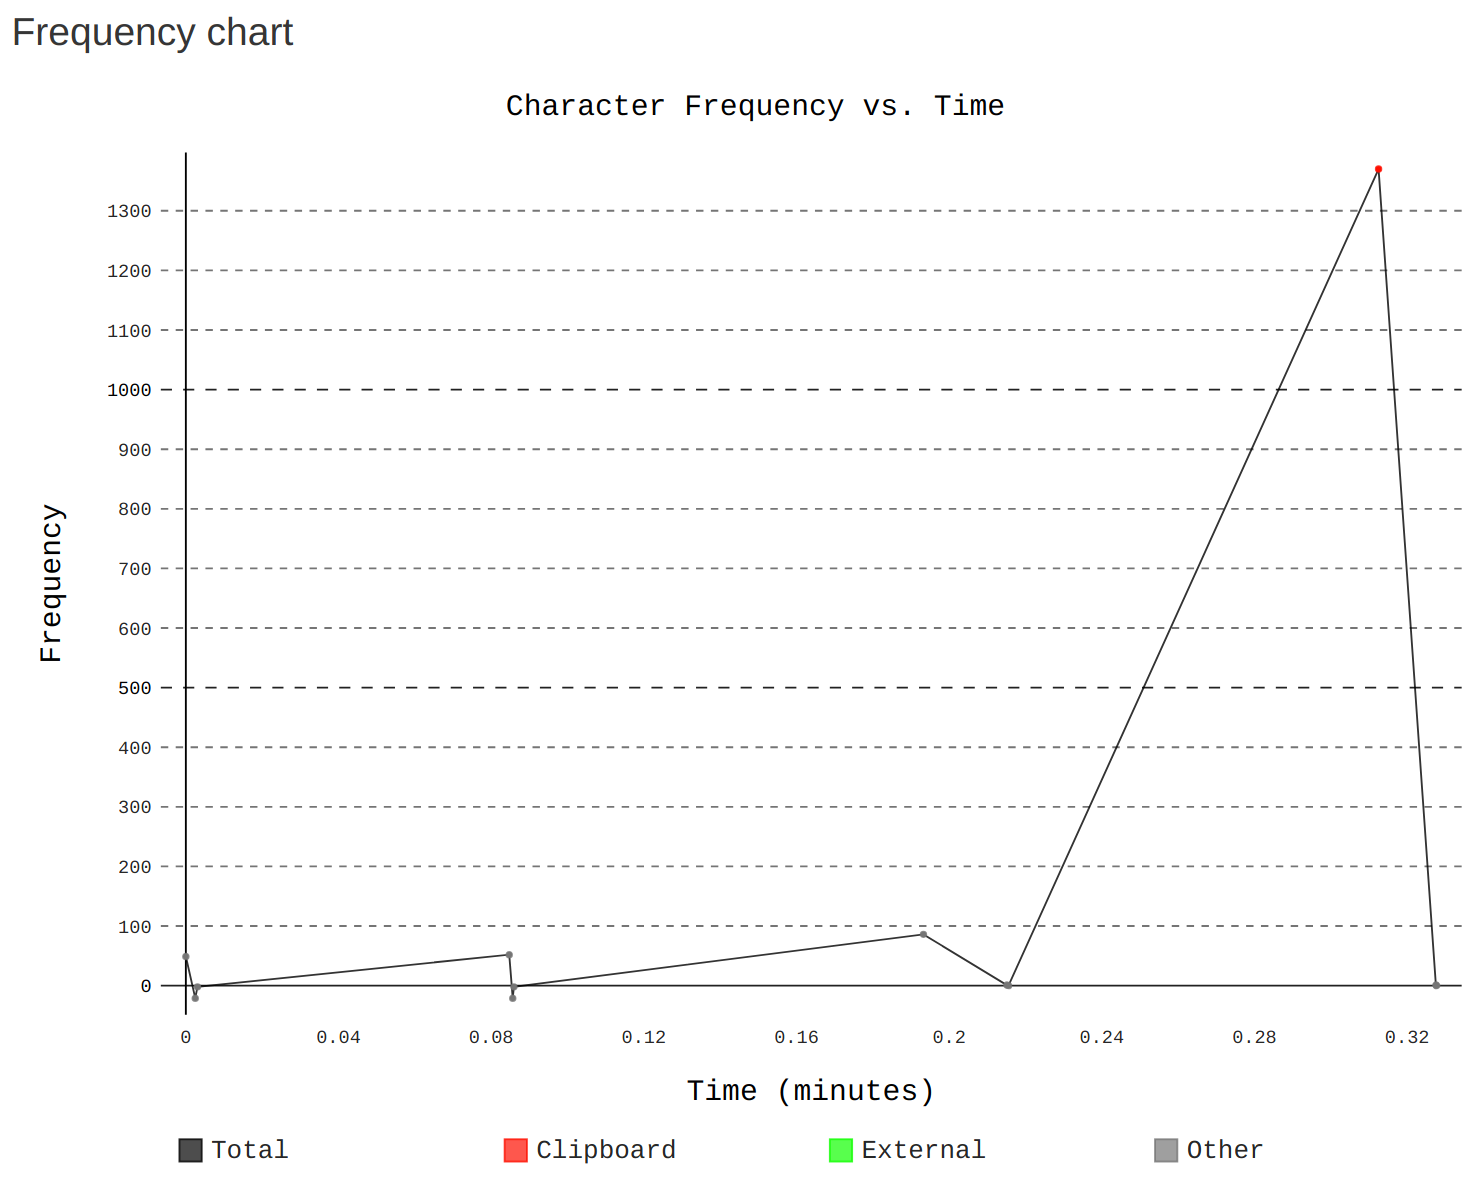
\includegraphics[height=.8\textheight,
    keepaspectratio=true,
    width=.8\textwidth,
    ]{figures/12-web-view-bad-submission-chart.png}
  }
  \caption[Web Submission FTS Chart]{An example submission FTS chart. This shows the type of source code changes over the development time of a submission.}
  \label{fig:web-submission-details-chart}
\end{figure}

\begin{figure}[H]
  \centering
  \fbox{
    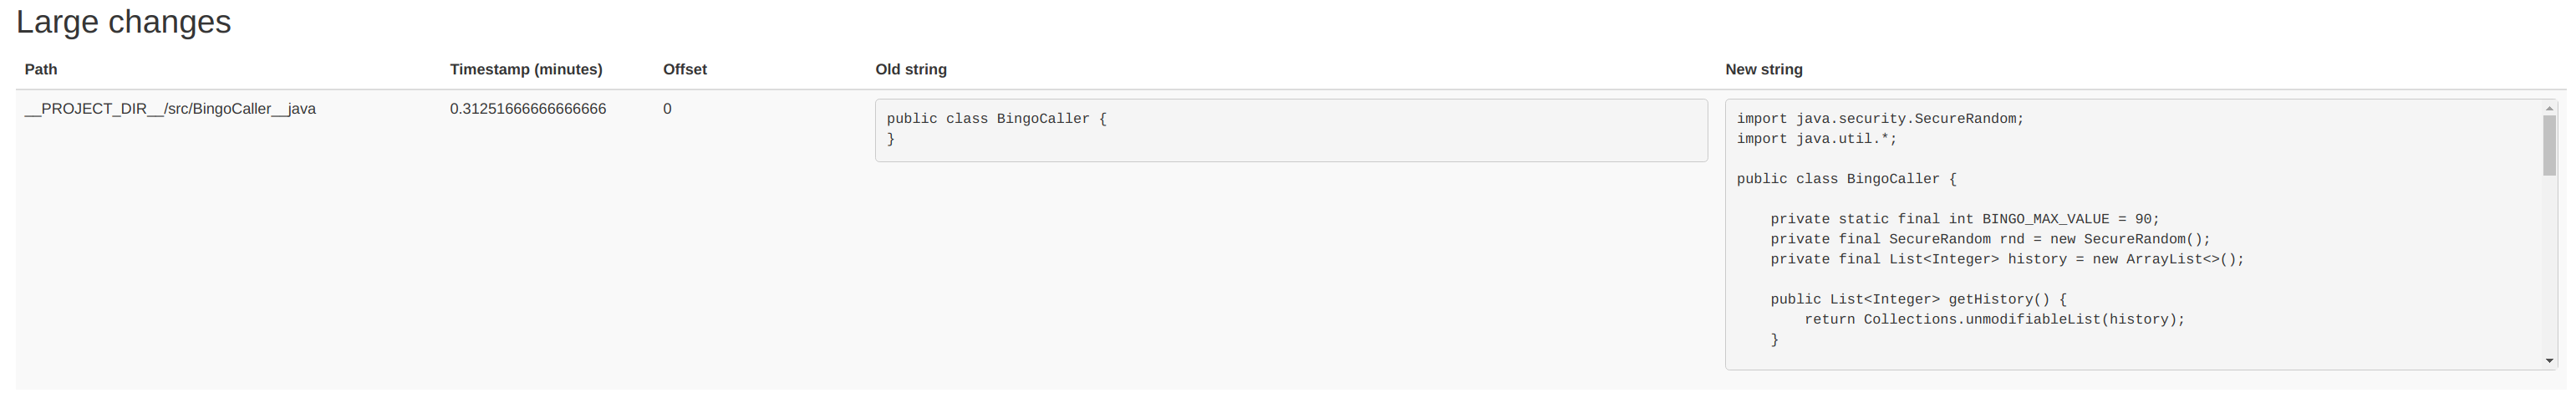
\includegraphics[height=\textheight,
    keepaspectratio=true,
    width=\textwidth,
    ]{figures/13-web-view-bad-submission-changes.png}
  }
  \caption[Web Submission Changes]{An example submission large changes. This shows the major changes tracked for a submission.}
  \label{fig:web-submission-details-changes}
\end{figure}

\newpage

\section{Docker Containers}
The back-end server and post-processor were both written with Docker in mind. Docker containers were used to easily deploy each of the server components. These components are the back-end server, post-processor, and database. Each of these have an individual \texttt{Dockerfile}. Docker Compose is used to seamlessly deploy all of these applications as separate containers with simple commands. See \autoref{cde:docker-compose} for the \texttt{docker-compose.yml} file. The mongodb service is built and deployed as a container first. This is because both the post-processor and server services depend on it. The local \texttt{data/db} directory is mounted to provide persistence for the database across deployments. This allows the container to stop and the data to remain on disk. The post-processor and server pass through the \texttt{PDP\_DEBUG} environment variable. This is used by both of the components to enable debug logging when the value is present. The server service mounts the local server directory to the container. This allows Flask to hot-reload when files are changed locally. This removes the need to restart all containers when small changes are made to the server code. Both the mongodb and server services open ports for the containers. This is required for mongodb so that other containers can connect to it. The server opens the port so users can access the web service.

%TC:ignore
\begin{code}
\begin{minted}[breaklines,
               linenos,
               frame=lines]{yaml}
version: '2'
services:
  mongodb:
    build: ./mongodb
    hostname: mongodb
    ports:
      - 27017:27107
    volumes:
      - ./data/db:/data/db
  postprocessor:
    build: ./postprocessor
    depends_on:
      - mongodb
    environment:
      - PDP_DEBUG=${PDP_DEBUG}
  server:
    build: ./server
    depends_on:
      - mongodb
    environment:
      - PDP_DEBUG=${PDP_DEBUG}
    ports:
      - 8000:8000
    volumes:
      - ./server:/plagiarism_detection/server
\end{minted}
\caption{The docker-compose.yml file. This file is used to deploy multiple containers with Docker Compose.}
\label{cde:docker-compose}
\end{code}
%TC:endignore

\autoref{cde:dockerfile-server} shows the Dockerfile for the back-end server. The Dockerfile uses the Python base image. This provides the basic Python infrastructure, including the Python interpreter and pip (both version 3). The working directory is configured and system requirements are installed (not pip requirements). The entrypoint script is added. The entrypoint script is executed when the container is created as it is defined as the entrypoint on L22. The requirements file is added and pip is used to install the requirements. L17 is used to add the current local directory to the working directory in the container. This will add the server files to the container. The unit tests are executed using nose. If any tests fail then the container will fail to build and will not run.

%TC:ignore
\begin{code}
\begin{minted}[breaklines,
               linenos,
               frame=lines]{dockerfile}
FROM python:3.6.4-slim

WORKDIR /plagiarism_detection/server

RUN apt-get update && \
    apt-get install -y gcc

ADD entrypoint.sh ./
RUN set -ex && \
    chmod +x entrypoint.sh

ADD requirements.txt ./

RUN set -ex && \
    pip3 install -r requirements.txt

ADD ./ ./

RUN set -ex && \
    nosetests --with-coverage --cover-erase --cover-package=server -v

ENTRYPOINT ["./entrypoint.sh"]
\end{minted}
\caption{The Dockerfile for the server}
\label{cde:dockerfile-server}
\end{code}
%TC:endignore

\autoref{cde:dockerfile-server-entrypoint} shows the entrypoint Bash script for the server as used by the Dockerfile above. This script simply executes the server as a Python module.

%TC:ignore
\begin{code}
\begin{minted}[breaklines,
               linenos,
               frame=lines]{bash}
#!/usr/bin/env bash

SCRIPT_DIR="$( cd "$( dirname "${BASH_SOURCE[0]}" )" && pwd )"

pushd ${SCRIPT_DIR} >/dev/null

python3 -m server
\end{minted}
\caption{The server Dockerfile entrypoint Bash script}
\label{cde:dockerfile-server-entrypoint}
\end{code}
%TC:endignore
